\documentclass{article}
\usepackage{multicol}
\usepackage{graphicx}
\usepackage[legalpaper, total={6in, 10in}]{geometry}
\usepackage{blindtext}
\usepackage{caption}
\usepackage{sectsty}
\usepackage[style=numeric,backend=bibtex]{biblatex}
% \usepackage[backend=biber]{biblatex}
\usepackage{hyperref}
\usepackage{setspace}

\addbibresource{refs.bib}

\title{Gravity}
\author{
  Amogh Param\\
  \texttt{aparam@cs.ucla.edu}
  \and
  Tushar Bhat\\
  \texttt{tushar@cs.ucla.edu}
}
\date{}

\begin{document}
  \sectionfont{\fontsize{12}{15}\selectfont}
  
  \maketitle

  \begin{multicols}{2}

  \section*{Abstract}  
	We present a novel approach to portable weight measurement and monitoring. Our approach involves embedding a shoe with an array of sensors that wirelessly communicate with a user's smartphone and provide an accurate measurement of weight. In addition, this system forms part of a platform for continuous weight monitoring and analytics.
  		
  \section{Introduction}
	Weight measurement has generally been restricted to large, stationary weight scales. Present day weight scales aren?t portable as they cannot be worn by a person and as result cannot provide a continuous weight measurement to the user. Consistent and more intensive self-weighing has been studied to help individuals catch weight gains before they escalate and also help make behavior changes to prevent additional weight gain \cite{cite1}. Another problem is that present day weight scales limit the frequency of weight measurements as they are not portable. Therefore, our objective was to build a portable weight measurement system that would help monitor the user?s weight consistently.\newline

	\noindent
	Changes in weight reflect changes in the healthiness of lifestyle. A sudden weight change in a short duration of time for a person may result from an illness or by following an extreme diet. Following such a diet has been studied to be unhealthy to the person \cite{cite2}. Weight loss can result from a decrease in body fluid, muscle mass, or fat. A decrease in body fluid can come from medications, fluid loss, lack of fluid intake, or illnesses such as diabetes. Some causes of weight loss include, but are not limited to, cancer, viral infection (such as CMV or HIV), gastroenteritis, parasite infection, depression, bowel diseases, and overactive thyroid (hyperthyroidism). Hence, having a consistent weight measurement system will help detect these unhealthy weight changes and promote the user to follow a better weight management strategy to lead a healthier lifestyle. \newline \newline 
	
	\noindent  
	We can further build a classification system to help correlate the rate of weight change associated with different types of illness or diets. \newline

	\noindent
	In this project however, we primarily focus on building the portable weight measurement system and provide a platform to collect, monitor and analyze user weight data.

	\subsection{Market research}
		A study that was done in \cite{cite3} shows that the global weight loss management market is expected to reach \$206.4 billion by 2019 from \$148.1 billion in 2014, growing at a CAGR (Compound Annual Growth Rate) of 6.9\%. Major factors driving the growth of this market include increase in obese population, strong government support and funding, lifestyle changes, increase in membership for health clubs, and most importantly technological advancements.\newline
		
		\noindent
		Another study in \cite{cite4} predicts that the fitness tracker market will hit about \$2.2 billion in 2015. In the study, they quote IHS technology as estimating that the worldwide revenue from sports, fitness and activity tracking devices will grow by about 46\% between 2013 and 2019. They attribute this growth to the increasing number of health-conscious consumers willing to buy wearable devices that help them manage and maintain a healthy lifestyle. 

	\subsection{Related Work}
		Over the years, there has been significant interest in the field of wearable devices embedded in the shoe. In \cite{cite8}, the authors considered building a shoe containing 2 scales entirely housed within its sole, where the scales may be deployed downward so that they project beneath the shoe's sole?making the scales thereby able to accurately weigh the wearer as the wearer briefly stands only upon the thus deployed scales. In \cite{cite9} the authors built an article of footwear having one or more sensors mounted in the shoe which, when impacted by an object, are effective to send a signal to a controller representative of the magnitude of the force with which the object was struck by the shoe. 

		\noindent
		In \cite{cite10}, the authors built a system that continuously monitors pressure and force on the foot, analyzes and visualizes the pressure and force exerted on the foot in real-time. The device measures pressure and force applied to an array of sensors placed in various points of an orthotic, shoe, shoe lining, insert, sock or sock type device. If the sensors detect force, they send a signal to a microprocessor located in the shoe that subsequently analyzes and sends the data wirelessly to either a handheld electronic device, a personal computer, an electronic data capture system or a software program. 


  \section{Approach}
  	Our primary objectives were to have a device which can be embedded in a shoe and be able to measure a voltage difference when a person stands on the device, wirelessly send sensor data to a mobile device and correlate the voltage to and predict the weight of the person, based on a mathematical regression model. Our approach to achieve our objective was to architect a system as shown in Figure 2.1.

	\begin{center}
	  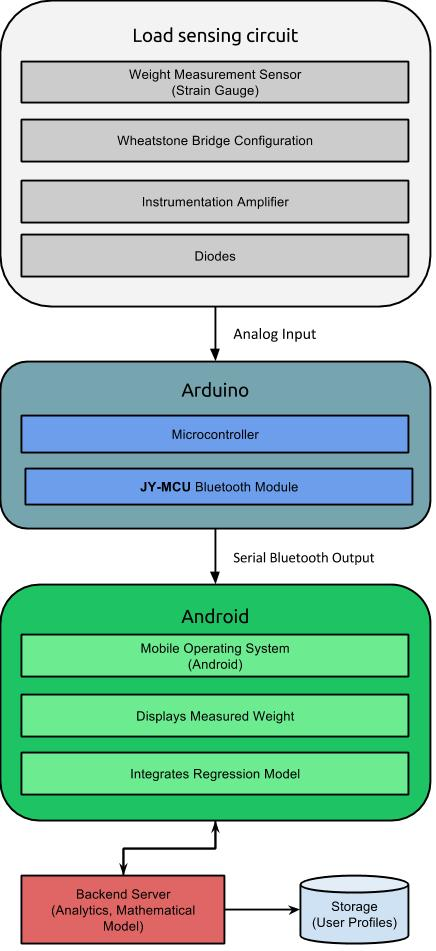
\includegraphics[height=135mm]{images/1_architecture.jpg}
	  \captionof{figure}{Architecture}
	\end{center}

	\noindent
	\subsection{Architecture}
	Our system architecture is built modularly to allow for extensibility. Each module performs one specific function and communicates an output to the next module of the architecture. We describe each part of the architecture  in the following subsections.

	\subsubsection{Load Sensing Circuit}
	The load sensing circuit forms the core circuitry for providing a way to measure the weight of the user. It works on the principle that as an increasing load is placed on a load cell, the voltage in the circuit changes. The difference between the base voltage (under no load) and the new voltage (under load of a specific weight) is measured and output to the the arduino module. This voltage difference is associated with the actual weight and our mathematical model is trained to learn the correlation of this voltage and the actual weight.

	\subsubsection*{Weight Sensors (Load Cells)}
	Weight sensors change their resistance when a force or pressure is applied to them. Therefore, these sensors behave as variable resistors in the load sensing circuit which in turn change the voltage in the circuit. As the amount of weight placed on the load cell increases, the amount of the voltage difference also increases. This voltage difference can thus give an accurate measure of the actual weight of the user. We primarily experimented with using two types of weight sensors/load cells as follows: 

	\paragraph{\textit{Force Sensitive Resistors}}
	Force-sensing resistors (FSR) consist of a conductive polymer that changes resistance when a force is applied to its surface \cite{cite5}. The sensing film consists of both electrically conducting and nonconducting particles suspended in a matrix. When a force is applied to the surface of the sensing film, the particles touch the conducting electrodes, thus, changing the resistance of the film. A major disadvantage of these FSRs is that although they provide good sensitivity, they are highly imprecise. 

	\paragraph{\textit{Strain Gauge}}
	A strain gauge (or strain gage) is a device used to measure strain on an object. As the object is deformed, an internal foil is deformed, causing its electrical resistance to change. The underlying principle is that when an electrical conductor is stretched within the limits of its elasticity such that it does not break or permanently deform, it will become narrower and longer, thus increasing its electrical resistance end-to-end.\newline 

	\noindent
	Conversely, when the conductor is compressed, it will broaden and shorten, thereby decreasing its electrical resistance end-to-end. From this measured electrical resistance of the strain gauge, and the corresponding voltage difference, the amount of applied stress may be inferred.\newline

	\noindent
	In our experiments, the strain gauge was more accurate than the Force-sensitive resistors and as a result, we integrated the strain gauge in our final design. Although using a strain gauge was better than using the FSR, the amount of voltage change that we were able to achieve by directly connecting the load cell into the circuit was extremely low. As a result, we used the strain gauge in a wheatstone bridge configuration to get a greater measurement for the changing voltage. 

	\paragraph{\textit{Wheatstone Bridge}}
	A typical Wheatstone bridge consists of four resistors positioned such that the current from the battery splits, flows through the configuration of resistors and then recombines into a single conductor. Three of the resistors in this circuit have static resistances and the fourth resistor is the load cell with variable resistance (based on the load placed on it). Using a wheatstone bridge provides a way to identify extremely small changes in resistance (in the variable resistor) by measuring the voltage difference across the ‘sensing’ terminals. This voltage difference increases or decreases as the weight on the load cell increases or decreases, respectively. This provides a way to accurately measure the weight on the load cell. \newline

	\noindent
	Although the output from the wheatstone bridge configuration is quite reliable and stable, the magnitude of the voltage difference measured across the ‘sensing’ terminals is extremely small (order of a few millivolts for ~50 lbs loads). As a result, we used an amplifier to amplify the voltage difference from the wheatstone bridge.

	\paragraph{\textit{Operational Amplifier (LM358N)}}	
	Operational amplifiers are DC-coupled high-gain electronic voltage amplifiers with a differential input and a single-ended output. The operational amplifiers produce an output voltage/potential that is typically many orders of magnitude larger than the voltage difference between its input terminals. LM358N is an integrated circuit consisting of dual low-power operational amplifiers. The voltage from the wheatstone bridge is fed into the amplifiers and a voltage gain is obtained at the output of the operational amplifier. This voltage is then used to infer the exact weight of the user. The LM358N op-amp however, has a lot of problems associated with it. \newline

	\noindent
	In our experiments, we found that the amplified voltage was extremely noisy. Although the input voltage was amplified, the voltage flux made it extremely hard to get an accurate voltage reading for a specific weight. As a result, we averaged the voltage fluctuations and collected data (during the training phase).\newline

	\noindent
	\textbf{\textit{Instrumentation Amplifier}}	
	The inherent problems with the LM358N op-amp lead us to use a more stable amplifier, INA125P (Instrumentation amplifier). We are currently running experiments with this amplifier and hope to have successful results.\newline

	\noindent
	\textbf{\textit{Diodes}}	
	The main function of diodes are to allow current to flow in one direction and prevent it from flowing back in the other direction. However, it also allows us to drop the voltage of the current flowing through it. As the Arduino’s input can only handle voltage between 0-5V, we used an array of diodes to drop the base voltage gain to ~1V. This voltage was then fed into the output of the Arduino.

	\subsubsection{Arduino}
	The Arduino microcontroller provides an interface to supply the amplified voltage difference from the load sensing circuit as input to one or more of its input pins. The microcontroller can thus measure the input voltage and communicate this measured voltage to the user’s smartphone via its serial outputs.	One important characteristic of the Arduino is that it provides a 10 bit output interface (i.e) the output values from the Arduino range from 0-1023 and as a result, we need to scale the voltage down to a range of 0-5V.\newline

	\noindent
	\textbf{\textit{JY-MCU Bluetooth Module}}
	The arduino microcontroller communicates with the smartphone via the JY-MCU bluetooth module. It provides an interface that allows the arduino to wirelessly communicate with the smartphone. The bluetooth module reads the serial output of the arduino and communicates it to the smartphone.
	
	\subsubsection{Android}
	We built an Android application that seamlessly integrates with the Arduino’s bluetooth interface. The application consists of the following components:\newline

	\noindent
	\textbf{\textit{ConnectToDeviceActivity}}		
	This Android activity provides an interface to search for nearby bluetooth devices and provides the required address information to the next activity to initiate the bluetooth socket connection.\newline

	\newpage
	
	\end{multicols}
	\begin{center}
	  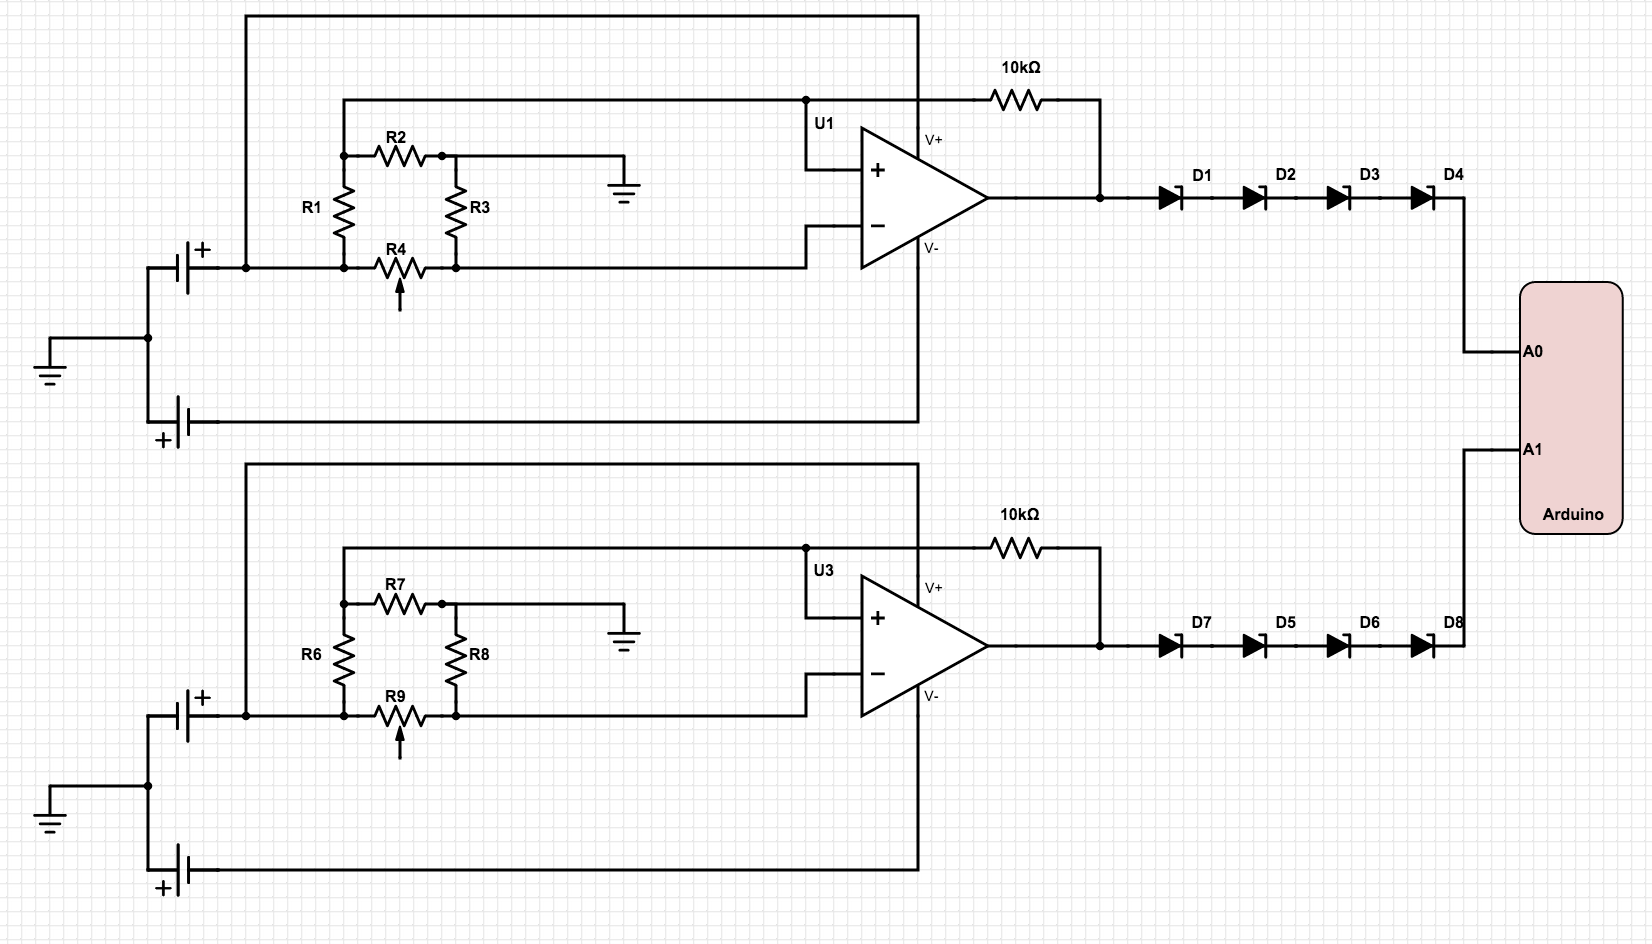
\includegraphics[height=80mm]{images/2_circuit.png}
	  \captionof{figure}{Circuit Schematic}
	\end{center}
	\begin{multicols}{2}	

	\noindent
	\textbf{\textit{MainActivity}}			
	This activity provides the main user interface and creates a socket with the bluetooth device. It displays the current voltage output by each of the operational/ instrumentation amplifiers and provides an interface to collect and label data for the mathematical model. The activity also displays the corresponding weight of the user using a mathematical model.

	\subsubsection{Sensor Placement}
	For our prototype we assume that the subject is standing on the shoes containing the sensors in a level area, with his/her line of sight parallel to the floor. This will ensure that the subject's center of gravity is positioned directly above his/her heels.

	\begin{center}
	  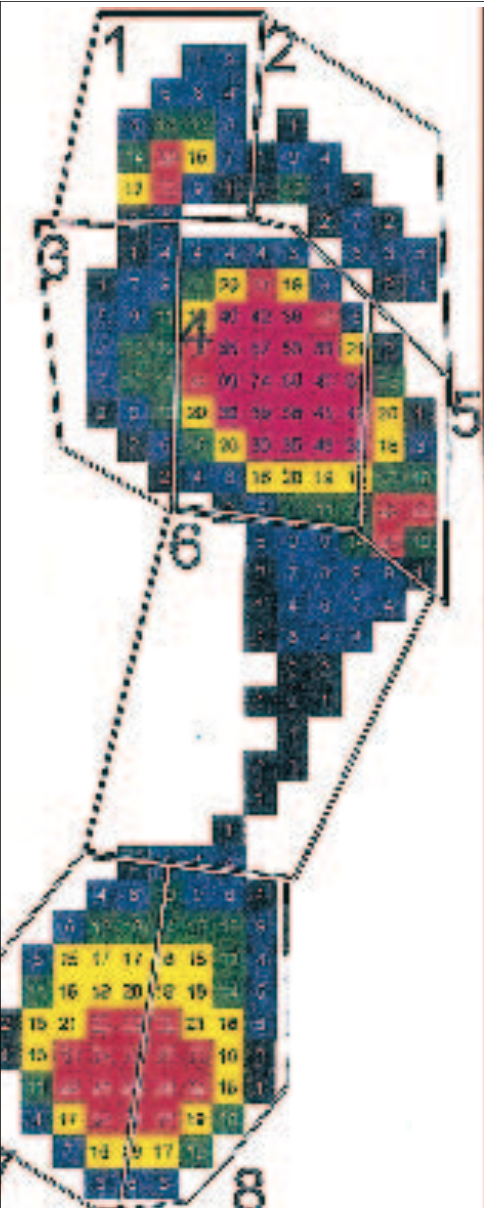
\includegraphics[height=50mm]{images/3_placement.png}
	  \captionof{figure}{Weight Distribution}
	\end{center}

	\noindent
	As seen in Figure 2.2 , most of the body weight, in this position, will be distributed between three areas, the heel, the metatarsals and the toes, with the toes supporting the least weight among the three areas. \cite{cite7}

	The prototype consists of one shoe sole, containing two sensors. One of sensors is placed under the heel area and the other is placed under the metatarsal area; both in as central a location to their respective regions as possible to ensure a proper measurement of weight.

	\subsubsection{Training (Data Collection)}
	Given a known weight, we set the current voltage as our base voltage (differential voltage reference of 0V). As stress is added onto the 2 load cells (strain gauges), the output voltage from the circuit increases. This voltage is fed into the arduino which then sends this voltage to the smartphone. The android application on the smartphone then uses the base voltage and finds the additional voltage gained due to the added stress. This additional voltage provides the voltage reference that signifies the weight added to the load sensors. 
	The application allows us to capture the voltage differential readings from both the sensors and label the known weight. The differential voltages across the two sensors and the target weight are written into a .CSV file on the device. We externally use the measurements in the .CSV file to derive a mathematical model to correlate the voltage differences to the weight.


	\subsubsection{Mathematical Model}
	To build the mathematical model, we’ve first manually label weights and collect corresponding sensor output values. Next, we plot these sensor output values against the labeled weights and fit a curve to the data scatter. The fitted curve will define a function that takes as input, the sensor outputs, and the output of this function will be the required weight.

  \section{Experiments}
  READ FROM CSV
  \newpage

  \section{Conclusion}
  In this paper, we propose a portable system architecture for weight measurement. The approach uses a load sensing circuit with embedded load cells (strain gauge sensors) connected to an arduino microcontroller with a bluetooth module. The arduino reads the voltage difference from the load sensing circuit and communicates it to the user's smartphone which in turn runs the voltage values against a mathematical model and predicts the user'��s weight. \newline

  \noindent
  We experimented using force sensitive resistors which were very inaccurate. As an alternative, we used strain gauge sensors which resulted in better measurements. As the voltage difference from the circuit was very small (order of mV) for large loads, we amplified the voltage with operational amplifiers and obtained higher voltage differences. However, the amplified voltage was extremely noisy and was constantly fluctuating to get a precise reading. Therefore, our solution was to average the voltage fluctuation and use the average as our reference voltage. This provided an almost linear correlation with the amount of weight placed on the load cells. Although, based on what the base voltage was set to, we tended to get extremely fluctuating readings. We observed that as long as the base voltage was almost stable, we got an almost linear relationship, but otherwise, we obtained data that was extremely noisy without any discernible pattern. 
  
  \section{Future Work}
  Our initial aim going forward is to improve the accuracy of our readings such that we can measure even minor changes in weight accurately. Assuming that we can build a set of sensors with an acceptable reading accuracy, there are multiple applications for the same. By adding extra pressure sensors across the sole of the shoe, we can measure distribution of weight across the foot and can notify the user when his/her posture is correct or if their style of walking/running is incorrect. We can also plot the user'��s weight fluctuation over time, allowing them to accurately judge the effectiveness of their fitness routines. We can also integrate with other sensors, such as heart-rate sensors, to directly correlate physical activity with weight loss over time and display the results to the user, and GPS location data, to analyze the weight gains at different locations. Based on sensor data we may also be able to classify the activity being performed by the user at any given time and offer analytics on user behavior.
  
  % \nocite{*}
  % \printbibliography

	\nocite{*}
	\begingroup
	\setstretch{1}
	\setlength\bibitemsep{10pt}
	\printbibliography
	\endgroup

  
  \end{multicols}  
\end{document}
